\setAuthor{Siim Ainsaar}
\setRound{piirkonnavoor}
\setYear{2011}
\setNumber{G 10}
\setDifficulty{7}
\setTopic{Geomeetriline optika}

\prob{Nõguslääts eestvaates}
Joonisel on kujutatud eestvaates nõguslääts, mille optiline peatelg on joonise tasandiga risti ja lõikub läätsega punktis $O$. Antud on ka üks horisontaalne valguskiir ning selle lõikepunktid eesmise fokaaltasandi ning läätsega (vastavalt punktid $K$ ja $L$). Joonestage antud vaates lisalehel kiire edasine käik ning lõikepunkt tagumise fokaaltasandiga. Põhjendage lahendust.
\begin{center}
	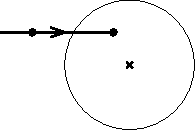
\includegraphics[width=0.5\linewidth]{2011-v2g-10-yl}
\end{center}

\hint
Kui nõgusläätsele langevad paralleelsed kiired, lõikuvad
murdunud kiirte pikendused eesmisel fokaaltasandil.

\solu
Kui nõgusläätsele langevad paralleelsed kiired, lõikuvad
murdunud kiirte pikendused eesmisel fokaaltasandil. Joonistame antud kiirega paralleelse abikiire (optilise kõrvaltelje, joonisel $AO$), mis läbib läätse optilist keskpunkti. See abikiir ei murdu, seega ühtib oma läätse läbimise järgse osa pikendusega. Tema lõikepunkti eesmise fokaaltasandiga (punkti $A$) leiame tõigast, et lõik $AO$ on lõigu
$KL$ paralleellüke. Küsitav murdunud kiir asub siis sirgel $AL$. Lääts asub täpselt oma
fokaaltasandite vahel keskel, seetõttu poolitab punkt $L$ lõigu $AB$, kus $B$ on küsitav murdunud kiire lõikepunkt tagumise fokaaltasandiga. Järelikult saame punkti $B$, kui peegeldame punkti $A$ punkti $L$ suhtes ($|AL| = |LB|$).

\begin{center}
	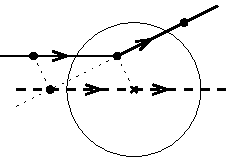
\includegraphics[width=0.5\linewidth]{2011-v2g-10-lah}
\end{center}
\probend